\documentclass[9pt,twocolumn,twoside,lineno]{pnas-new}
% Use the lineno option to display guide line numbers if required.

\templatetype{pnasresearcharticle} % Choose template 
%{pnasresearcharticle} %= Template for a two-column research article
% {pnasmathematics} %= Template for a one-column mathematics article
% {pnasinvited} %= Template for a PNAS invited submission

\title{Retinal neuronal ensembles encode  properties of natural images}

% Are natural images encoded by neural assemblies in the retina

% Use letters for affiliations, numbers to show equal authorship (if applicable) and to indicate the corresponding author

\author[b]{Jes\'us P\'erez-Orthttps://www.overleaf.com/project/5e878bbd7076dc000132cfa4ega}
\author[a]{Joaqu\'in Araya}
\author[a]{Cristobal Ibaceta}
\author[a]{Rub\'en Herzog}
\author[c]{Mar\'ia-Jos\'e Escobar}
\author[d]{Fernando Peña-Ortega}
\author[d]{Luis Carrillo-Reid}
\author[a]{Adrian G. Palacios}

\affil[a]{Centro Interdisciplinario de Neurociencia de Valparaiso, Facultad de Ciencias, Universidad de Valparaiso, Valparaiso, Chile}
\affil[b]{Department of Biological Sciences, Columbia University, New York, USA}
\affil[c]{Departamento de Electrónica, Universidad Técnica Federico Santa María, Valparaíso, Chile}
\affil[d]{Instituto de Neurobiología
UNAM, Juriquilla, Querétaro, Mexico}

% Please give the surname of the lead author for the running footer
\leadauthor{Lead author last name} 

% Please add a significance statement to explain the relevance of your work
\significancestatement{Authors must submit a 120-word maximum statement about the significance of their research paper written at a level understandable to an undergraduate educated scientist outside their field of speciality. The primary goal of the significance statement is to explain the relevance of the work in broad context to a broad readership. The significance statement appears in the paper itself and is required for all research papers.}

% Please include corresponding author, author contribution and author declaration information
\authorcontributions{Please provide details of author contributions here.}
\authordeclaration{Please declare any competing interests here.}
\equalauthors{\textsuperscript{1}A.O.(Author One) contributed equally to this work with A.T. (Author Two) (remove if not applicable).}
\correspondingauthor{\textsuperscript{2}To whom correspondence should be addressed. E-mail: author.two\@email.com}

% At least three keywords are required at submission. Please provide three to five keywords, separated by the pipe symbol.
\keywords{Retinal Neural Coding $|$ Neuronal Ensembles $|$ Visual System $|$} 

\begin{abstract}
Please provide an abstract of no more than 250 words in a single paragraph. Abstracts should explain to the general reader the major contributions of the article. References in the abstract must be cited in full within the abstract itself and cited in the text.
\end{abstract}

\dates{This manuscript was compiled on \today}
\doi{\url{www.pnas.org/cgi/doi/10.1073/pnas.XXXXXXXXXX}}

\begin{document}

\maketitle
\thispagestyle{firststyle}
\ifthenelse{\boolean{shortarticle}}{\ifthenelse{\boolean{singlecolumn}}{\abscontentformatted}{\abscontent}}{}

\dropcap{N}euronal ensembles correspond to a group of neurons sequentially activated by a concomitant order of firing \citep{Carillo-Reid, Yuste 2020} supporting brain neural coding \citep{RN2970, RN3475, RN3476, Hebb:1961vs} \textbf{[Carillo-Reid, Yuste 2020, REF Here]}. However,  sensory systems still missing explicit studies on the presence, structure, functionality and dynamic of neuronal ensembles. The retina, a piece of central nervous system, in the back of the eye, integrates photon flux trough a well-organized multilayer neural network \citep{Gollisch:2010kv}, \citep{Wassle:2004jy}  formed by a variety of retinal ganglion cells (RGCs), classified according its morphology \citep{Sanes:2015fe},  physiology \citep{Farrow:2011gi} and genetics profile \citep{Sumbul:2014hs}. The  collective behavior of RGCs  \citep{Nirenberg:2001hy} specially neural synchrony \citep{Levine:1998wu, Mastronarde:1983io, Mastronarde:1983dt, Mastronarde:1987hg, Barlow:2001ub, Shannon:1998ti}, has been propose to sustaining neural coding for, e.g., for gratings \citep{Hochstein:1976vr}, sensitivity to movement \citep{Hammond:1982uk, Frost:1983vf, Born:1992kz}, approaching \citep{Munch:2009hy} and differential movement \citep{Olveczky:2003ka}. The advent of multi-electrode array devices (MEA) \citep{Meister:1995jc}, suggest that retinal population coding involve sophisticated and modular neural networks architectures \citep{Smirnakis:vu, Manookin:2006gl, Greschner:2011fk, Vidne:2011is, Trenholm:us, Sharpee:2007de, Gollisch:2010kv, Maffei:1973hh, MOVSHON:1979fv}. 

The retinal architecture is tuned by  the collective properties of a rich and diverse variety of photoreceptors, bipolar, horizontal, amacrine cells, and RGCs integrate these signals to respond to, e.g., movement, direction, color or light intensity. Cats visual cortex showed an exquisitely functional receptive field (RF) architecture, sensitive to orientation and direction \citep{Rose:1977fg}, with clear functional advantage \citep{Ohki:2005ce}. The visual cortex of rats respond to the repetition of a moving grid or under a natural movie presentation with a well organized reverberating spatiotemporal patterns response \citep{Han:2008hw}. Carillo et al. \citep{CarrilloReid:2015fm}, has shown that groups of neurons are sequentially activated by time patterns triggered by a specific visual stimuli, e.g., a natural image or the movement of a bar in different directions, indicating that brain microcircuits encode visual aspects changing over time. Moreover, several other studies strongly suggest that cortical activity is drive by a group of co-active synchronously neurons \textbf{[REF REVIEW HERE]}. Miller \citep{Miller:2014eq} described several principles to define such co-activation or neuronal ensembles: intrinsic “spontaneous ensembles” overlap with “evoked ensembles”; light pattern – moving bar or natural movie – evoke neuronal ensembles that are locked to “spontaneous” observed neuronal ensembles.
These results suggests that neuronal ensembles are active either  spontaneously or can be recruited when relevant visual stimuli are presented. Furthermore, some active neurons are either "promiscuous" - less specialized- they participate to more than one neuronal ensemble, whether other are "specialized" and participate in only one neuronal ensemble for a specific behavior. Although the concept of neuronal ensemble has been present for years, is less known concerning How neuronal synchronous activity is generated by a particular stimulus? How neuronal ensembles are built in time ? What is their ultimate functionality for the neural code? \citep{CarrilloReid:2016jn, CarrilloReid:2015fm}. To approach such questions Here we study the retina of \textit{Octodon degus}, a diurnal dichromat visual rodent \citep{Chavez:2003bn}.

\subsection*{Results}
\subsection*{Natural stimulus evoked neuronal ensembles}
The collective behavior of RGCs was evoked by different visual stimuli and recorded with a MEA technique (see methods). In Figure 1A we show a schematic setup and in 1B the stimuli used (full field): scotopic or dark stimulus; photopic or light (cyan) stimulus; white noise (cyan and dark) and a natural movie (cyan) (60 Hz) corresponding to a 30 sec sequence of a video recorded in the natural environment of O.degus. In Figure 1C (top) a representative raster plot is shown where each row correspond to a single RGC, isolated using a spiking sorting algorithm (see methods), in function of each stimulus used. Figure 1C (bottom) correspond to the co-activity level of an active number of RGC during a particular stimuli presentation. How we can see the neuronal co-activity, as well the spike rate in Figure 1D, is stimulus dependent, with an increase for the natural movie. 

\begin{figure}
\centering
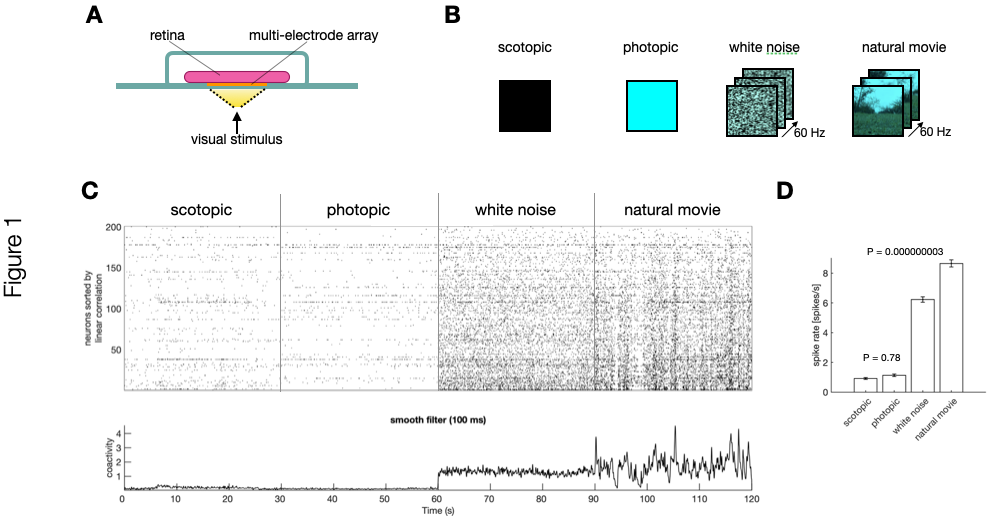
\includegraphics[width=9 cm,height=9cm]{Fig 1.png}
\caption{A) correspond to a schematic set-up for the MEA recording. B) Different stimulus used: scotopic, photopic, white noise and natural movie. C) A representative raster plot for RGCs responses for different stimuli (Top) and  the corresponding associated neural co-activity (Bottom). D) spike rate for different stimuli}
\label{fig:Figure_1.png}
\end{figure}

\subsection*{Consecutive images in natural stimulus produce the activation of retinal neuronal ensembles}
The natural movie stimulus evoked sequential and high co-activity peaks compared to any other stimulus used here. Figure 2A, shows a representative experiment where we plotted the raster plot for the 1st, 2nd, 3rd, 4th, 20th and 40th trial. Each neuronal raster reproduce a very close pattern of RGCs response along the trials. Figure 2B represent the neural co-activity of different groups of RGCs (sequential colors) forming different neuronal ensembles that fire together depending on the structure of the visual contents. 

% In Figure 2A RGCs were sorted according to their correlation with the co-activity signal (Figure 2B), i.e. the first neuron is the most correlated and the last neuron is the least correlated. Note that not correlated neurons appears to remain their activity during different stimuli (top neurons of Figure 2A). 

Co-activity signal clearly shows those differences (Figure 2B) as well as the evoked simultaneous activation of groups neurons (co-activity peaks): scotopic and photopic stimulus evoked few co-activity peaks; during the white noise and natural movie stimulus, the basal co-activation incremented, although the last generated co-activity peaks with greater amplitude. To determine a single threshold of co-activity peaks, in all stimuli, the basal co-activity were adjusted by subtracting its own average \textbf{(Figure XXX, see Materials and Methods)}. For each co-activity peak we obtained a neural vector and then we computed Euclidean similarity between them \textbf{(equation 1, Figure XXX)}. The number of different neural states were identified using hierarchical cluster analysis between all neural vectors \textbf{(Figure XXXX)}, the different states were differently colored in Figure 2B. 

%Unexpectedly, similar population co-activity, or same neural state, was evoked during in scotopic, photopic and white noise stimuli. Although the white noise stimulus produced more co-activation peaks, all of them were from the same neural state.

Nevertheless, the natural movie stimulus evoked different population co-activity along the movie, i.e. a sequence of different neural states that would be encoding the frames of the scene. We counted the number of co-activity peaks and different states in all stimuli in 4 animals, natural movie stimulus significantly evoked more neural states than scotopic, photopic and white noise stimuli (\textbf{REF P=?, Figure 2G-H}). Therefore, retinal ensembles, are only evoked by the natural movie stimulus.

%Then, we obtained a neural vector for each co-activity peak (see Materials and Methods, Figure 1C, right). 

\begin{figure}
\centering
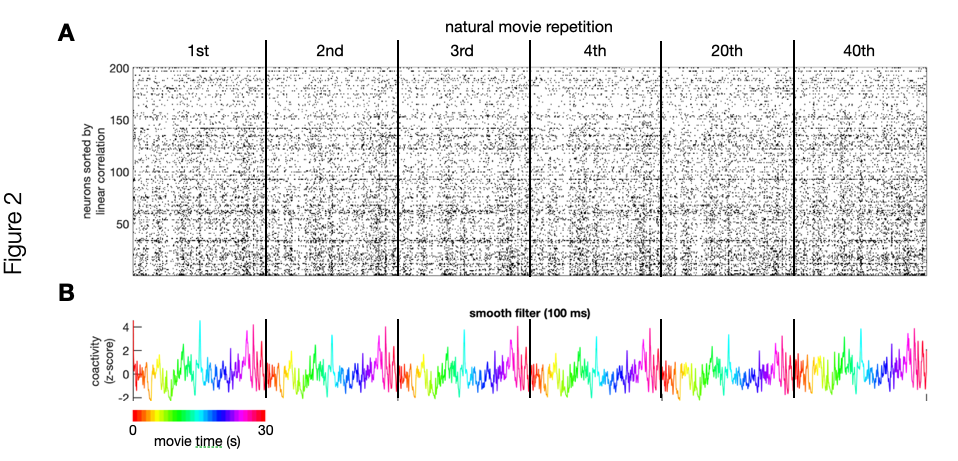
\includegraphics[width=8cm,height=8cm]{Fig 2.png}
\caption{A) representative raster plot for the 1st, 2nd, 3rd, 4th, 20th and 40th trial each of 30 sec duration. In B) the neural co-activity of different groups of RGCs (sequential colors) forming different neuronal ensembles. }
\label{fig:Figure_2.pdf}
\end{figure}

\subsection*{Retinal ensembles encode a natural sequence}

Since the retinal ensembles are so precise, we asked about the dependency between evoked retinal ensembles with the sequence or order of frames presentation during the natural movie. RGCs were stimulated the natural movie during 20 consecutive trials with its original order (left panel), then 20 consecutive trials but played backward with frames in an inverted order (middle panel). We were very careful to extract the exact times of each stimulation. At first glance it seems to evoke a similar neural activity (Figure 3A and 3B). 

%Continuous neural vectors were created for the 40 stimulus using time window of 1 s as it was the most precise. We defined 30 neural states using hierarchical clustering (Figure 7B-D), in order to get the same sequence and its reversed sequence. 
The neural state sequence from the same stimulus repetition (normal or played backwards) was as precise as we observed before, but unexpectedly, the neural state sequences between played forward and backward natural stimuli were very different (Figure 3E). Because the co-activity peaks seemed similar between forward and backward natural stimuli, maybe the difference was due to a time shift (despite extracting the exact times). The co-activity signal from the 1st and the 20th repetition of each stimulus was very similar, but the first repetition between both stimulus was little similar (Figure 3). The Pearson correlation coefficient between co-activity signals was measured (Figure 3). Between repetitions of the same stimulus, the correlation coefficient was above 0.9, but between forward and backward stimulus the correlation coefficient was below 0.4. Clearly, retinal ensembles encoded differently the same natural movie stimulus depending if it was played forward or backward. 
Then, we asked whether the consecutive images in the natural movie stimulus were the responsible of the retinal ensembles activation. To test for, we carried an experiment where the frames of the natural movie were shuffled \textbf{[DEFINITION HERE]} and the result shows the lost of co-activation observed before. First, we stimulated with the same frames from the natural movie, but shuffling the projection order of each frame (shuffle movie, Figure 3A). Despite being the same frames, the co-activity peaks were not generated as the same amplitude than in the natural order (shuffle movie, Figure 3B).
In Figure 3B we shows a high level of co-activation comparable for the first two conditions, where in the third condition we observe a much lower co-activation suggesting that the original order of the frames, where  movements, accelerations, stops, occurred as when an animal explore its natural environment mater to created a particular ensemble of RGCs. 

\textbf{Explain Here}
In Figure 3C we shows the results from different experiments same experiments with the respective average (in z-score). Figures 3D and 3E \textbf{[EXPLAIN]}

Figure 3C shows values of co-activation for n experiments for the natural movie (top), inverted movie (middle) and shuffle movie (bottom) conditions. \textbf{Figure 3D Figure 3E}


\begin{figure}
\centering
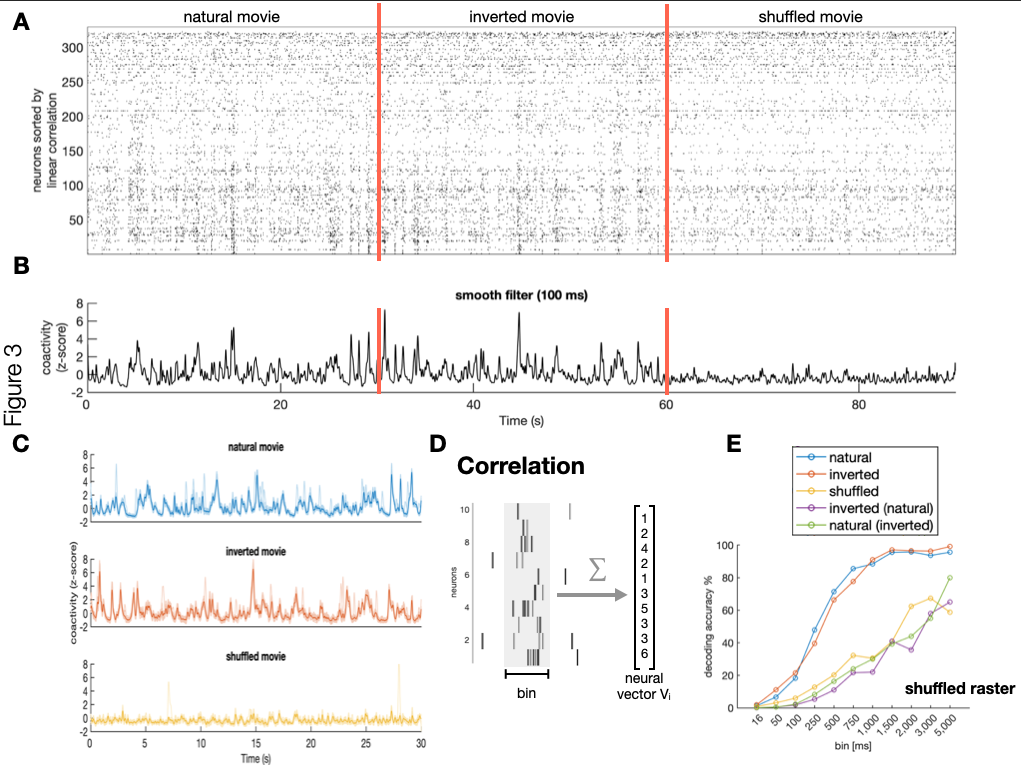
\includegraphics[width=8cm,height=9cm]{Fig 3.png}
\caption{A) raster plot for a natural movie experiment with its frames: original order (left panel), inverted order (middle panel) and shuffle order (right panel). B) co-activation level (z-score) for the third condition. C) co-activation value for the natural movie (top), inverted movie (middle) and shuffle movie (bottom) condition. \textbf{Figure 3D Figure 3E}}
\label{fig:Figure_3.pdf}
\end{figure}

%The shuffled stimulus lost the variety of neural states evoked during the natural stimulus (Figure 4A,B). Then we ask how many consecutive frames were needed to observe a retina ensemble. We shuffled and stimulated again with the same frames but keeping packs of 1, 2, 3, 4, 5 and so on, with consecutive frames (“shuffle 1", “shuffle 2”,..., “shuffle 5”, respectively; Figure 4C). Although all shuffle stimulation generated peaks of co-activity, none achieved, on average, the amplitude of co-activity peaks evoked by the natural movie stimulus (Figure 4A,B,C). However, while more consecutive images were used in the stimulation, the RGCs began to generate co-activity peaks of greater amplitude. Five consecutive images seems to be necessary to trigger a co-activity level comparable to the one evoked by the natural movie.

\begin{figure}
\centering
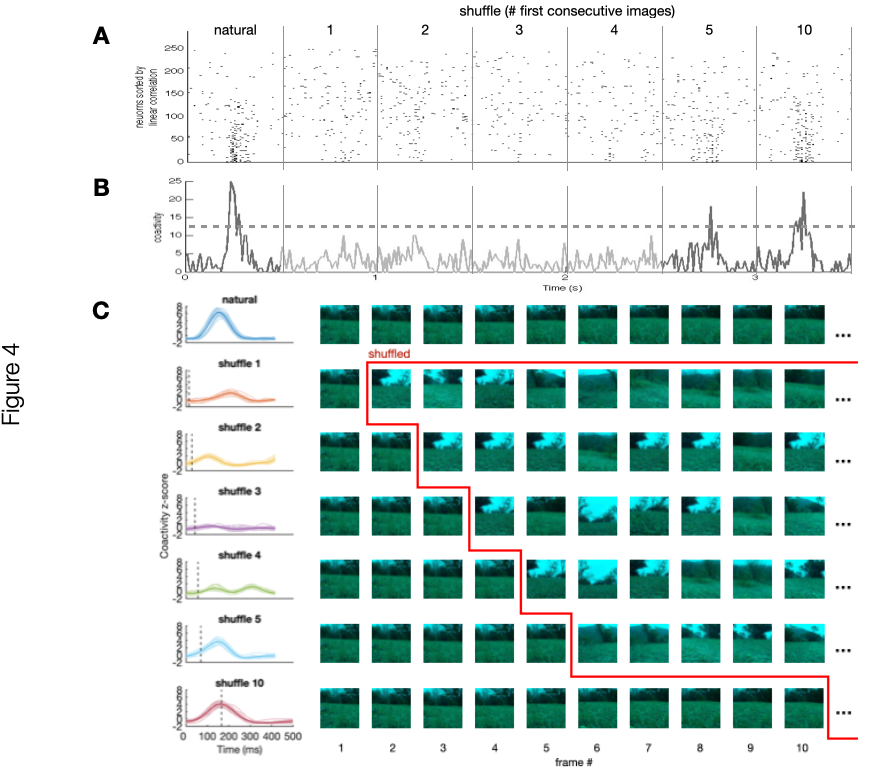
\includegraphics[width=8cm,height=9cm]{Fig 4.png}
\caption{REF}
\label{fig:Figure_4.pdf}
\end{figure}


%\subsection*{Electrical coupling is crucial for activating neural ensembles in the retina}
%In order to know if retinal ensembles depends on electrical coupling, we applied 18-beta-Glycyrrhetinic acid (BGA), a connexon blocker (Contreras et al., 2003), to the bath during the natural movie stimulus (Figure 3A right). We observed not only a decrements in activity, also a decrements in number and amplitude of co-activity peaks (Figure 3B), and the remaining co-activity peaks belong to the same neural state evoked by white noise stimulus (Figure 3C-D). The sequence of neural states produced by natural movie stimulus was abolished by the application of BGA. The count of co-activity peaks and different neural states were significantly reduced by the application of BGA (P=?, Figure 3E-F). As in Figure 2A, neurons in raster plot were sorted according to their correlation with the co-activity signal. Most of the neurons decreased their activity with BGA, but the neurons that increased their activity were not correlated with the co-activity peaks (Figure 3G). We distinguished the cell type of all neurons (see Materials and Methods) in 3: ON, OFF, and unknown cells. The OFF cells are more correlated with the co-activity peaks than the ON and unknown cells (Figure 3H). The largest proportion of cells that decreased their activity with BGA were the OFF cells, while the largest proportion of cells that increased their activity were ON and unknown cells (Figure 3I-J).

\subsection*{It takes ~80 ms of a natural stimulation to evoke a significant co-activation}
As we observed, the significant co-activation of the RGCs did not depend on the images per se, but on the natural sequence of them. Then, we asked how many consecutive frames generates a distinctive co-activity peak. We take 30 frames (500 ms) from the natural movie that evoked a co-activity peak and we shuffled all of them (“shuffle”), then we kept the first 1, 2, 3, 4, 5, 10 consecutive frames from the natural stimulus and original order (Figure 4A) and the rest of single frames were shuffled, without keeping consecutively. There was no response until 5 consecutive images of natural stimulus, producing a significant co-activity peak (Figure 4B). We obtained the neural vectors with a time window of 500 ms (per stimulus), in this case the neural vectors were not defined by significant peaks on co-activity signal. The Euclidean similarity between vectors were measured and clustered in 2 groups (Figure 4C left). The neural vectors evoked by 5 and 10 consecutive images were identified similar to the vector evoked by natural stimulus (Figure 4B). The Euclidean similarity increased until 5 consecutive natural images stimulus \textbf{(Figure 4 XX)}. In our experimental conditions, 5 consecutive images from a natural stimulus were projected in ~83.3 ms, therefore this time is necessary to evoke a significant co-activity peak.

\subsection*{Retinal ensembles encode the natural movie stimulus with high precision}
Consecutively images in the natural movie trigger retinal ensembles activation. Our next question was: Did the repetition of natural movie produce similar retinal ensembles activation? To answer this question we stimulated the RGCs with the same natural movie (30s at 60 Hz) for 20 times \textbf{(Figure 6)}. Neural vectors were created with a continuous windows of 1 s, 760, 500, 200, 100 and 60 ms. Natural movie duration was 30 s,  i.e. 30 neural vectors were obtained for windows of 1 s, 60 neural vectors for windows of 500 ms, and so on. For each time window size, the activity evoked of the 20 repetitions of the natural stimulus were analyzed together, and clustered in different neural states depending of the number of vectors created (v.g., for windows of 1 s, 30 neural states were defined using hierarchical clustering; \textbf{Figure 6A-E)}. To compute precision, we compare the state sequence between the 1st natural movie stimulus and the ith repetition. We expected similar sequence of neural states between different repetitions of the natural stimulus, but not so precisely (~100\%) as we observed for all the experiments with windows of 1 s (n = 5; Figure 6E). Even for windows of 200 ms, the precision of the neural state sequences of the 20 repetitions were above 8\% (Figure 6F and 6H). For time windows of 60 ms, the precision decreased below 50\%, thereby as the time window was reduced, the precision was also reduced (Figure 6G-H).

\begin{figure}
\centering
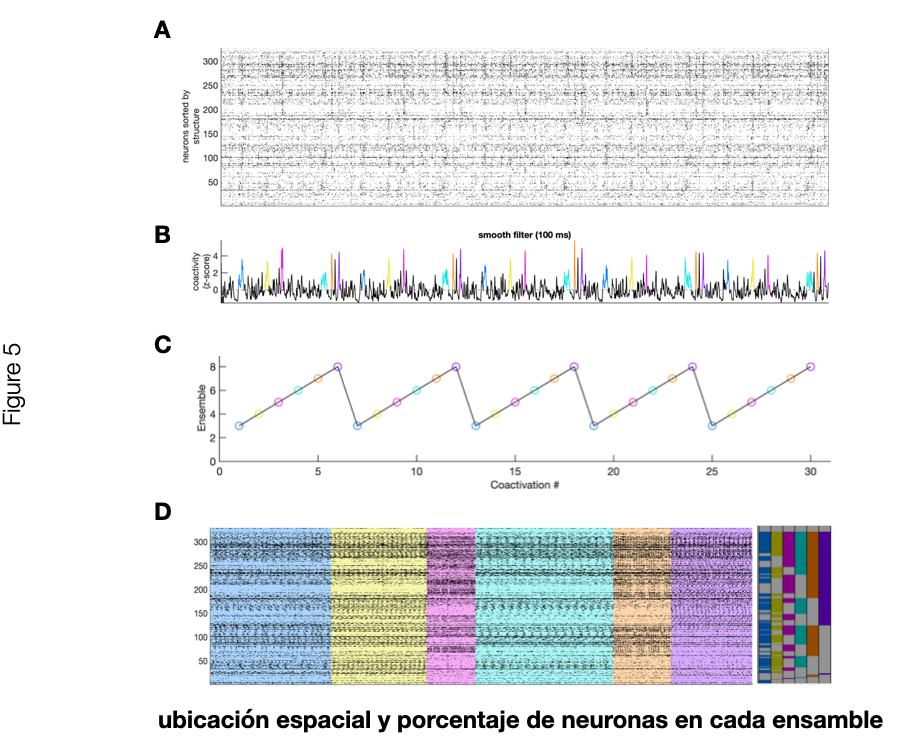
\includegraphics[width=9cm,height=9cm]{Fig 5.png}
\caption{REF}
\label{fig:Figure_5.pdf}
\end{figure}


\subsection*{Discussion}
Buzsáki suggested that neural ensembles would be organized into first order and higher order relationships, after syntactic rules known by both the sending cell (encoding) and the receiving (decoding) \citep{Buzsaki:2010jh}. If inputs to a system produce the same activity pattern repeatedly, the set of active elements that make up that system will have a more robust inter-association \citep{Buzsaki:2004bi}. That is, each element (e.g., cell or neuron) will tend to activate other cells and (with negative weight) to inactivate cells that are not part of the network pattern. The latter assumption is close to the mechanism postulate for neural plasticity. In other words, the observed pattern response will become 'self-associated,' or in others terms a memory pattern of "engram" \citep{Hebb:1961vs}. For example, at the microcircuit level, the cortex is dominated by excitatory connections, with a high density of interconnections, a reverberating activity could link individual neurons within functional neuronal clusters \citep{RN3482}.

 These neuronal ensembles are collectively activated by sensory inputs forming a short-closed interconnected circuit that acts in the absence of external stimulation \citep{RN3487}. Furthermore, the stimulation of a few members of that ensemble can activate the whole ensemble, as well as a cascade of neighboring other ensembles\textbf{ (REF)}.


%\subsection*{Author Affiliations}

%Include department, institution, and complete address, with the ZIP/postal code, for each author. Use lower case letters to match authors with institutions, as shown in the example. Authors with an ORCID ID may supply this information at submission.

%\subsection*{Submitting Manuscripts}

%All authors must submit their articles at \href{http://www.pnascentral.org/cgi-bin/main.plex}{PNAScentral}. If you are using Overleaf to write your article, you can use the ``Submit to PNAS'' option in the top bar of the editor window. 

%\subsection*{Format}
%Many authors find it useful to organize their manuscripts with the following order of sections;  title, author line and affiliations, keywords, abstract, significance statement, introduction, results, discussion, materials and methods, acknowledgments, and references. Other orders and headings are permitted.

%\subsection*{Manuscript Length}

%A standard 6-page article is approximately 4,000 words, 50 references, and 4 medium-size graphical elements (i.e., figures and tables). The preferred length of articles remains at 6 pages, but PNAS will allow articles up to a maximum of 12 pages.

%\subsection*{References}

%\begin{SCfigure*}[\sidecaptionrelwidth][t]
%\centering
%\includegraphics[width=11.4cm,height=11.4cm]{frog}
%\caption{This legend would be placed at the side of the figure, rather than below it.}\label{fig:side}
%\end{SCfigure*}

%\subsection*{Digital Figures}

%EPS, high-resolution PDF, and PowerPoint are preferred formats for figures that will be used in the main manuscript. Authors may submit PRC or U3D files for 3D images; these must be accompanied by 2D representations in TIFF, EPS, or high-resolution PDF format. Color images must be in RGB (red, green, blue) mode. Include the font files for any text.

%Images must be provided at final size, preferably 1 column width (8.7cm). Figures wider than 1 column should be sized to 11.4cm or 17.8cm wide. Numbers, letters, and symbols should be no smaller than 6 points (2mm) and no larger than 12 points (6mm) after reduction and must be consistent. 

%Figures and tables should be labelled and referenced in the standard way using the \verb|\label{}| and \verb|\ref{}| commands.

%Figure \ref{fig:frog} shows an example of how to insert a column-wide figure. To insert a figure wider than one column, please use the \verb|\begin{figure*}...\end{figure*}| environment. Figures wider than one column should be sized to 11.4 cm or 17.8 cm wide. Use \verb|\begin{SCfigure*}...\end{SCfigure*}| for a wide figure with side legends.

%\subsection*{Tables}
%Tables should be included in the main manuscript file and should not be uploaded separately.

%\subsection*{Single column equations}

%Authors may use 1- or 2-column equations in their article, according to their preference.

%To allow an equation to span both columns, use the \verb|\begin{figure*}...\end{figure*}| environment mentioned above for figures.

%Note that the use of the \verb|widetext| environment for equations is not recommended, and should not be used. 

%\begin{figure*}[bt!]
%\begin{align*}
%(x+y)^3&=(x+y)(x+y)^2\\
      % &=(x+y)(x^2+2xy+y^2) \numberthis \label{eqn:example} \\
     %  &=x^3+3x^2y+3xy^3+x^3. 
%\end{align*}
%\end{figure*}


%\begin{table}%[tbhp]
%\centering
%\caption{Comparison of the fitted potential energy surfaces and ab initio benchmark electronic energy calculations}
%\begin{tabular}{lrrr}
%Species & CBS & CV & G3 \\
%\midrule
%1. Acetaldehyde & 0.0 & 0.0 & 0.0 \\
%2. Vinyl alcohol & 9.1 & 9.6 & 13.5 \\
%3. Hydroxyethylidene & 50.8 & 51.2 & 54.0\\
%\bottomrule
%\end{tabular}

%\addtabletext{nomenclature for the TSs refers to the numbered species in the table.}
%\end{table}

%\subsection*{Data Archival}

%PNAS must be able to archive the data essential to a published article. Where such archiving is not possible, deposition of data in public databases, such as GenBank, ArrayExpress, Protein Data Bank, Unidata, and others outlined in the \href{https://www.pnas.org/page/authors/journal-policies#xi}{Information for Authors}, is acceptable.


%\subsection*{Supporting Information Appendix (SI)}

%Authors should submit SI as a single separate SI Appendix PDF file, combining all text, figures, tables, movie legends, and SI references. PNAS will publish SI uncomposed, as the authors have provided it. Additional details can be found here: \href{https://www.pnas.org/page/authors/format#Supporting_Information}{policy on SI}. The PNAS Overleaf SI template can be found \href{https://www.overleaf.com/latex/templates/pnas-template-for-supplementary-information/wqfsfqwyjtsd}{here}. Refer to the SI Appendix in the manuscript at an appropriate point in the text. Number supporting figures and tables starting with S1, S2, etc.

%Authors who place detailed materials and methods in an SI Appendix must provide sufficient detail in the main text methods to enable a reader to follow the logic of the procedures and results and also must reference the SI methods. If a paper is fundamentally a study of a new method or technique, then the methods must be described completely in the main text.

%\subsubsection*{SI Datasets} 

%Supply .xlsx, .csv, .txt, .rtf, or .pdf files. This file type will be published in raw format and will not be edited or composed.

\matmethods{
The experimental protocol for MEA recording has been described before and follows~\citep{PalaciosMunoz:2014gi}.
\subsection*{Animals}\label{subsec:animals}
\textit{Octodon degus} born in captivity at the animal facility in the Universidad de Valparaiso, were maintained in a light and temperature controlled with \textit{ad-libitum} access to food and water. Dark adapted animals, for 30 min  were deeply anesthetized with isoflurane and beheaded. Experimental procedures were approved by the Institutional Committee on Bioethics for Animal Research from the University and in accordance with the bioethics regulation of the Chilean National Agency for Research and Development (ANID).
Degus are crepuscular / diurnal rodents with a high number \SI{30}{\%} of cones supporting a diurnal dichromatic vision ~\citep{Chavez:2003bn,Jacobs:2003dd}.
\subsection*{Electrophysiological recordings} %\label{subsec:electrophy}
Retinal ganglion cells (RGCs) responses were obtained using a Multi Electrode Array device  ~\citep{Segev:2004cu} (USB MEA256, 256MEA 100 or 200 /30iR-ITO, Multichannel Systems GmbH, Reutlingen, Germany) sampling at \SI{20}{kHz}. For recording a small piece of retina was mounted on a dialysis membrane array under perfusion with AMES medium bubbled with 95\% 0\textsubscript{2} + 5\% C0\textsubscript{2} at 33 \textdegree \text{C} and the pH adjusted to 7.4. 

\subsection*{Visual Stimulus}
For stimulus display a DLP projector  using custom optics to reduce and focus the image onto the photoreceptor layer, projecting from the RGCs side was used. The size of a pixel onto the photoreceptor layer was $\approx 4.7 \mu m$ and an average irradiance of $70 nW/mm^{2}$. The peak spectral emission of the DLP LEDs have peak emission at 460 nm and 520 nm (USB4000 Fiber Optic Spectrometer, Ocean Optics), both in the range of covers the dichromatic, green and the UV cones, vision of \textit{O.degus}~\citep{Chavez:2003bn}. A natural movie that reproduce the natural environment of O.degus was obtained using a small telecommanded four wheels device, home built, with a mounted camera (Go-Pro) allowing  pre-programmed displacement with smooth scanning up, down, left, right, slow, fats movements to emulate natural displacement of degus exploration in nature ~\citep{Vasquez:2020} Spike sorting analysis were performed using \textit{Spyking-Circus}~\citep{Yger:2018hy}.

\subsection*{Obtaining co-activity}
Timestamps of unitary recordings at 20 kHz from MEA were used to build a binary matrix R of size N x S, where N is the number of neurons and S the number of samples, representing time. In R matrix, 1 represents if a neuron has at least one spike and 0 if not in a given time. The bin resolution was 20 ms or 50 samples per second (we also use bin resolution of 1, 5 and 10 ms, see Figure 4). The number of active neurons in each sample were counted (sum of columns of R matrix), obtaining the co-activity vector (1 x S), or co-activity signal. The co-activity was smoothed with a moving average filter of 100 ms to detect easily peaks of co-activity \MJ{we should indicate we got no time-shift in the filtered signal}. If the co-activity signal has different basal levels between stimuli, co-activity signal is adjusted by subtracting its own average per stimulus.

\subsection*{Defining neural states}
We considered significant co-activity peaks that are above a threshold (P < 0.01) of the signal. The threshold is determined generating surrogate shuffled raster \citep{CarrilloReid:2015fm, RN3517}. Time-shift shuffle were used, where all neurons preserve their firing pattern but each one with a different temporal shifting. We generated 1,000 shuffled raster and their cumulative distribution function (CDF) of their co-activity, then the number of co-active neurons at the value of 0.99 of the CDF was taken as the threshold. The null hypothesis is that activity of neurons is independent and then the co-activity occurs randomly.
Spikes in a given significant co-activity peak were counted for each neuron and converted to a neural vector V of size N $ \times $ 1 \citep{RN3518}. To identify if neural vectors were produced by the same activation of neurons, the Euclidean similarity matrix S of size P $ \times $ P were computed for all vectors $(V_1,V_2, \dots ,V_P)$: where P is the number of vectors and delta is the Euclidean distance. Then, similarity matrix were used in a hierarchical cluster analysis using Ward linkage (this kind of linkage had the best faithfulness of the consistency in our hierarchical trees). To determine the number of clusters, or different neural states, we used the contrast function (\textbf{REF Beggs  Plenz, 2004)}.

\subsection*{Shuffling frames of natural movie}
To test if the sequence of frames in the natural movie were responsible for the evocation of significant co-activity peaks we stimulated the retina with the same frames but shuffling the order of apparition every 5 seconds. In shuffle 1, all frames were shuffled with resolution of 1 frame. In shuffle 2, all frames were shuffled with resolution of 1 frame too, except the first two consecutive frames. In shuffle 3, all frames also were shuffled with resolution of 1 frame, except the first three consecutive frames, and so on with shuffle 4, 5, 10 and 20.

\subsection*{Efficiency in the neural states sequence repetition}
Efficiency of two sequences of neural states, obtained by different repetition of the stimulus, is used here as the fraction of coincidence along the sequence. For example, for the 2 sequences: [1, 2, 3, 4] and [1, 2, 3, 1], the fraction of coincidence is 3/4. For many repetitions of the stimulus, the efficiency presented is the average of efficiency between all sequences of neural states.
}

\showmatmethods{} %Display the Materials and Methods

\acknow{This work was supported by grants from ICM-Chilean Science Millennium Institute grant P09-022-F. PLEASE ADD}

\showacknow{} % Display the acknowledgments section

\subsection*{References}
% Bibliography
\bibliography{pnas-sample}
\end{document}
